\section{DEVELOPMENT PROCESS \hrulefill}

The software development process used for this project is based the Open Unified
Process (OpenUP), a part of the Eclipse Process Framework \cite{EclipseND}. The
reasoning behind this choice is that, as a Rational Unified Process derivative,
OpenUP offers an open source process framework which is targeted at agile
development in small teams and provides a number of development phases and
activities which can be used when designing the project plan (Figure
\ref{fig:sequence-openup}).

\begin{figure}[H]
\centering
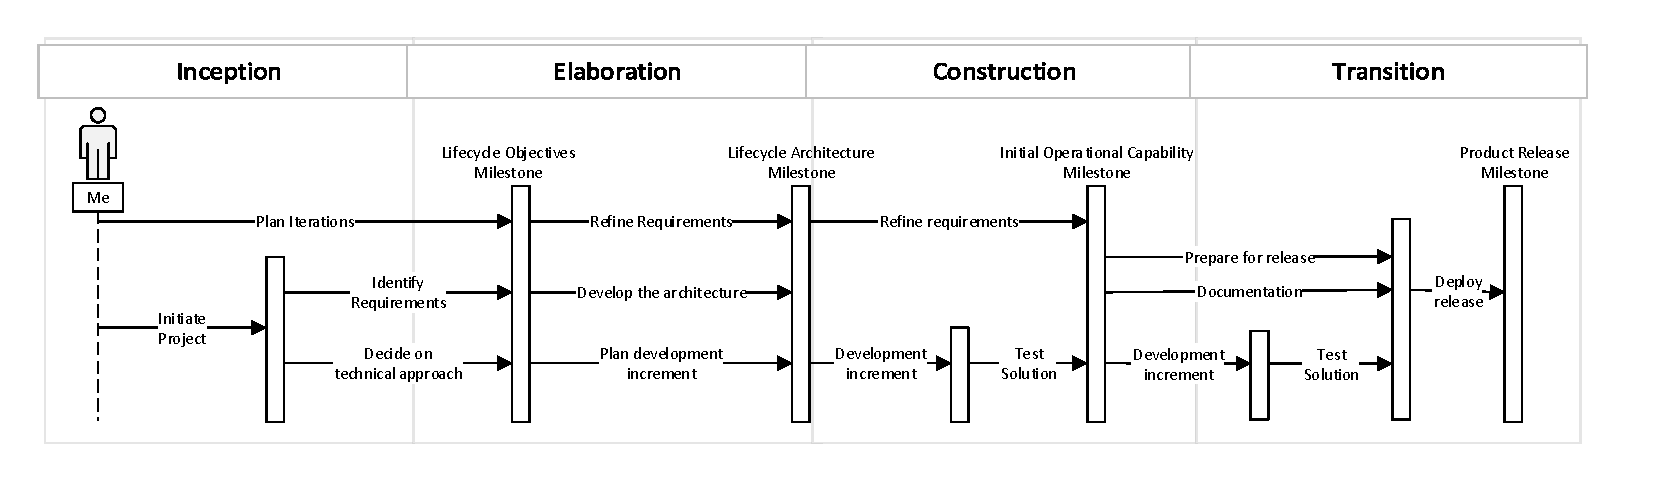
\includegraphics[width=7.5in]{assets/sequence-openup.pdf}
\caption{A sequence diagram showing a single full iteration of the OpenUP
  process}
\label{fig:sequence-openup}
\end{figure}

\subsection{Work Breakdown Structure}
The crux of OpenUP is in breaking down a large development project into four key
phases to iterate on: the Inception Phase, Elaboration Phase, Construction Phase
and Transition Phase \cite{Rational2011}.

\paragraph{Inception Phase} The inception phase represents the initial work
which defines the scope and objectives of the project. Key tasks include
generating a list of the core project's requirements, key features and main
constraints, and developing an understanding of the general project use-cases
and business case. The work in this phase culminates with a stakeholder
concurrence on the project scope, cost and schedule, and a deep requirements
understanding which covers the depth and breadth of the technical work to be
undertaken. For this project, the inception phase should include meeting all
project stakeholders and research into existing protein databases, their
use-cases, and a deeper understanding of the scientific value of the dataset.

\paragraph{Elaboration Phase} The elaboration phase builds upon the work done in
the construction phase by requiring deeper technical research into required
technologies, and initial prototyping of early ideas. By the end of the
elaboration phase, the product vision should be agreed upon and stable, and a
full plan of the technical architecture should have been reached.  Further
iterations of the elaboration phase may be used after construction has begun to
refine the architecture plan, or as a response to a change in the technologies
used. The purpose of the phase is to turn the initial product vision into a
realisable goal with quantifiable and achievable goals and objectives. For this
project, the elaboration phase will involve investigation into some of the
available technologies (PHP, MySQL, Node.js, MongoDB, etc.), and technical
prototypes of the database backend.

\paragraph{Construction Phase} The construction phase covers the development of
the main software architecture and associated documentation, and should result
in ``Initial Operational Capability'' (7). Success criteria for this development
phase includes whether the product is mature enough to be deployed to users, and
so for this project will require meeting with stakeholders to ensure that the
implementation of the plan is acceptable.
%TODO: ref

\paragraph{Transition Phase} The transition phase includes beta testing of the
new system against user expectations, and includes a review of the completed
product against the requirements and objectives established in the initial
project plan to measure success. The phase culminates in a product roll-out and
the associated distribution, marketing and training of users that is
required. For this project, it will involve deploying the finished project to a
public server and conducting extensive user testing.

\subsection{Version Control}

A revision control and source code management (SCM) system will be used during
all development to keep an auditable and transparent log of progress, and Git
will be used for this. There are numerous advantages that Git has over other
SCMs, chiefly that it is entirely open source and GPL licensed \cite{FSF1991},
it has a very lightweight branching model and good support for rebasing and
merging, and there are numerous sources which offer free hosting of open source
licensed projects that are tracked by Git. A public repository of the source
code and all relevant documentation for this project is available on GitHub
\cite{Cummins2013}.

\subsubsection{Issue Tracker}

One of the additional benefits of the GitHub online repository hosting service
is that it supplies a number of useful tools, namely an issue tracker and
milestones list. This allows issues to be created online and categorised
appropriately (e.g. bugs, tasks, regressions, documentation, etc.), and then
referenced from the repository commits.  Milestones can be created and
individual issues assigned to them, allowing for quick and visible progress
checking of development towards a specific goal.

\subsubsection{Test Driven Development}

By combining the available issue tracker with good version control practises, it
is possible to implement a simple and functional test driven approach to
development (Figure \ref{fig:flow-tdd}). This breaks down the development
process into single-issue chunks, with each iteration beginning with creating a
local development branch for an issue and then writing failing test cases which
can then be patched. Using this model of development ensures that all work
undertaken is relevant to the project and directly affects progress, minimising
the amount of time wastage and increasing the stability of the codebase by
ensuring adequate test coverage \cite{Martin2011}.

\begin{figure}[H]
\centering
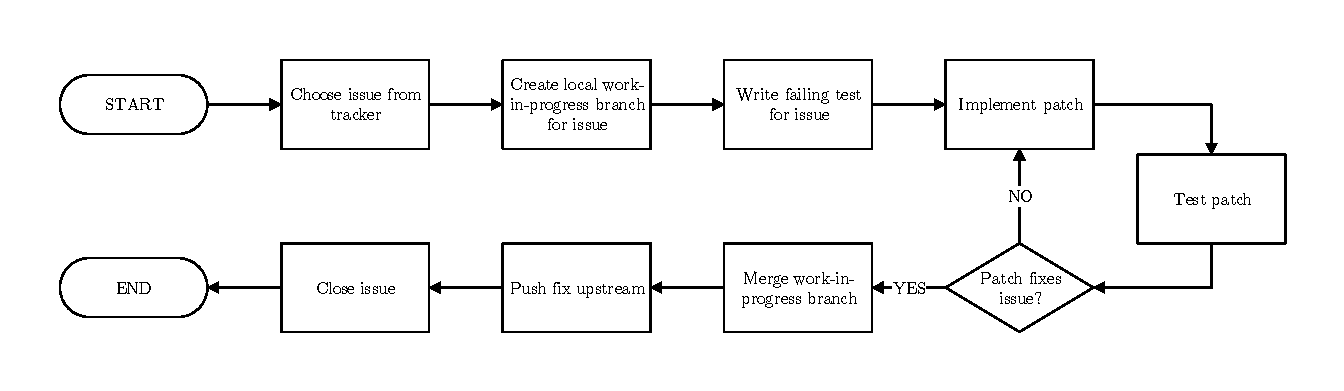
\includegraphics[width=7.5in]{assets/flow-tdd.pdf}
\caption{A single iteration of the project's test-driven development workflow}
\label{fig:flow-tdd}
\end{figure}
